\documentclass[a4paper]{article}\usepackage[]{graphicx}\usepackage[]{color}
%% maxwidth is the original width if it is less than linewidth
%% otherwise use linewidth (to make sure the graphics do not exceed the margin)
\makeatletter
\def\maxwidth{ %
  \ifdim\Gin@nat@width>\linewidth
    \linewidth
  \else
    \Gin@nat@width
  \fi
}
\makeatother

\definecolor{fgcolor}{rgb}{0.345, 0.345, 0.345}
\newcommand{\hlnum}[1]{\textcolor[rgb]{0.686,0.059,0.569}{#1}}%
\newcommand{\hlstr}[1]{\textcolor[rgb]{0.192,0.494,0.8}{#1}}%
\newcommand{\hlcom}[1]{\textcolor[rgb]{0.678,0.584,0.686}{\textit{#1}}}%
\newcommand{\hlopt}[1]{\textcolor[rgb]{0,0,0}{#1}}%
\newcommand{\hlstd}[1]{\textcolor[rgb]{0.345,0.345,0.345}{#1}}%
\newcommand{\hlkwa}[1]{\textcolor[rgb]{0.161,0.373,0.58}{\textbf{#1}}}%
\newcommand{\hlkwb}[1]{\textcolor[rgb]{0.69,0.353,0.396}{#1}}%
\newcommand{\hlkwc}[1]{\textcolor[rgb]{0.333,0.667,0.333}{#1}}%
\newcommand{\hlkwd}[1]{\textcolor[rgb]{0.737,0.353,0.396}{\textbf{#1}}}%

\usepackage{framed}
\makeatletter
\newenvironment{kframe}{%
 \def\at@end@of@kframe{}%
 \ifinner\ifhmode%
  \def\at@end@of@kframe{\end{minipage}}%
  \begin{minipage}{\columnwidth}%
 \fi\fi%
 \def\FrameCommand##1{\hskip\@totalleftmargin \hskip-\fboxsep
 \colorbox{shadecolor}{##1}\hskip-\fboxsep
     % There is no \\@totalrightmargin, so:
     \hskip-\linewidth \hskip-\@totalleftmargin \hskip\columnwidth}%
 \MakeFramed {\advance\hsize-\width
   \@totalleftmargin\z@ \linewidth\hsize
   \@setminipage}}%
 {\par\unskip\endMakeFramed%
 \at@end@of@kframe}
\makeatother

\definecolor{shadecolor}{rgb}{.97, .97, .97}
\definecolor{messagecolor}{rgb}{0, 0, 0}
\definecolor{warningcolor}{rgb}{1, 0, 1}
\definecolor{errorcolor}{rgb}{1, 0, 0}
\newenvironment{knitrout}{}{} % an empty environment to be redefined in TeX

\usepackage{alltt}
% setting very small margins
\usepackage{fullpage}
\IfFileExists{upquote.sty}{\usepackage{upquote}}{}

\begin{document}

\title{``Global signal" simulation}
%\author{Ellis Patrick with modification from Jean}
\maketitle

\begin{knitrout}
\definecolor{shadecolor}{rgb}{0.969, 0.969, 0.969}\color{fgcolor}\begin{kframe}


{\ttfamily\noindent\color{warningcolor}{\#\# Warning: package 'ggplot2' was built under R version 3.1.1}}\end{kframe}
\end{knitrout}


\section{Abstract}

\subsubsection*{Background}
Global Signal normalisation/correction/modelling/removal is a step often performed in fMRI analysis to remove/model signal in the bold that appears to be affecting all voxels. It had been hypothesised that this ``global signal" could be being driven by a particular region of the brain and should be accounted for in a similar way that cardiovascular and respiration effects are. 

\subsubsection*{Methods}
We will use simple simulations to evaluate three approaches for identifying connections/assocations between voxels in the brain. The simulations consider a scenario where there is no global signal and a scenario where there is a super-imposed  uniform global signal. The three approaches that will be assessed are correlation, partial correlation and correlation after global signal removal. These approaches will be evaluated using density plots and ROC plots. The density plots demonstrate each methods ability to capture the true simulated associations while the ROC plots assess the capability of each method to separate the true non-zero assocations from the non-existant ones. In terms of network construction, the latter is often more important than the former.

\subsubsection*{Conclusions}
We have demonstrated that global signal removal can have adverse effects to the interpretation of correlations between voxels. This is demonstrated in simulations with and without a super-imposed global signal. Specifically, global signal regression can shift true zero correlations to be negative. 





\section{A simplified brain.}

In order to understand the effects of global signal removal we will consider a simple abstract model of a brain.
We will start by assuming that our brain can be divided up into forty voxels. However these voxels will potentially interact with each other. For simplicity we will assume that these voxels interact in such a way that they can be divided up into four independent sub-networks. In two of the sub-networks the voxels will have pairwise correlations of 0.4, in two pairwise correlations of 0.2 and elsewhere zero. The correlation matrix can then be constructed in a block structure as shown in Figure \ref{fig:BlockMatrix}.

\begin{knitrout}
\definecolor{shadecolor}{rgb}{0.969, 0.969, 0.969}\color{fgcolor}\begin{figure}[]


{\centering 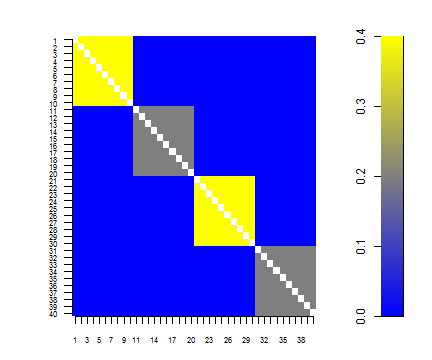
\includegraphics[width=0.7\textwidth]{GSFigs/GSBlockMatrix} 

}

\caption[A 2D representation of the correlation matrix that will be used to simulate correlated BOLD signals]{A 2D representation of the correlation matrix that will be used to simulate correlated BOLD signals. The correlation matrix consists of four sub-networks. The correlations within these subworks are uniformly either 0.4 or 0.2. All correlations between voxels outside of these sub-networks are zero. \label{fig:BlockMatrix}}
\end{figure}


\end{knitrout}


\section{Simulations}
In all of the following, a series of simulated BOLD signals will be generated.  A Multivariate normal distribution is used to generate 1000 observations of the 40 voxels, where the expected values of all voxels are 100 and covariance matrix equal to the correlation matrix as described in Figure \ref{fig:BlockMatrix}.

\subsection{No global signal}
The first simulation is a simulation where no global signal has been superimposed over the true correlation structure. Figure \ref{fig:DensityNoGS} plots the densities of the empirical correlations, partial correlations and correlations after GS removal. In this figure it can be observed that all of the global signal correlations have been shifted in a negative direction. However, while these correlations have been shifted they still separate into the correlations that were 0, 0.2 and 0.4 in the true correlation matrix. Here we also observed that while the empirical partial correlations are centered around their true values, their spreads are such that there is some overlap in their densities. This is an illustration of the variability introduced when trying to estimate partial correlations, as while the correlations only use information from two voxels, the partial correlations use information from all of the voxels.
 

\begin{knitrout}
\definecolor{shadecolor}{rgb}{0.969, 0.969, 0.969}\color{fgcolor}\begin{kframe}


{\ttfamily\noindent\itshape\color{messagecolor}{\#\# Loading required package: grid}}\end{kframe}\begin{figure}[]


{\centering 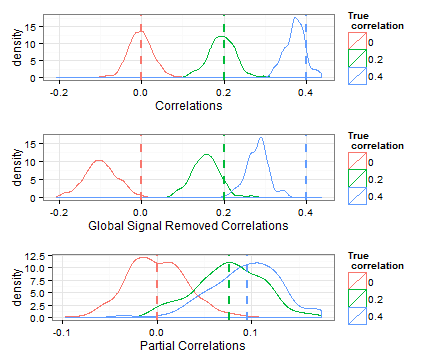
\includegraphics[width=\maxwidth]{GSFigs/GSDensityNoGS} 

}

\caption[The densities of the empirical correlations, partial correlations and correlations after GS removal are plotted for a simulation without a superimposed global signal]{The densities of the empirical correlations, partial correlations and correlations after GS removal are plotted for a simulation without a superimposed global signal. Correlations are labelled as to whether they were 0, 0.2 or 0.4 in the true correlation matrix that was used to generate them.\label{fig:DensityNoGS}}
\end{figure}


\end{knitrout}


To further assess the ability of each method to recapture the truth the empirical correlations, partial correlations and correlations after GS removal are plotted against the true correlations or parital correlations in Figure \ref{fig:dotPlotNoGS}.  In this figure it can be observed that while the empirical correlations and partial correlations do a good job of recovering the truth, the correlations after global signal removal have been shifted in a negative direction. In addition to the this the correlations with true correlation 0.4 have shifted further than those with true correlation 0.2.

\begin{knitrout}
\definecolor{shadecolor}{rgb}{0.969, 0.969, 0.969}\color{fgcolor}\begin{figure}[]


{\centering 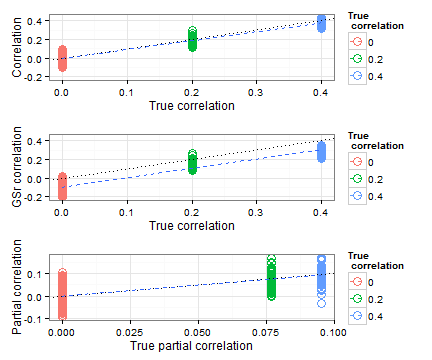
\includegraphics[width=\maxwidth]{GSFigs/GSdotPlotNoGS} 

}

\caption[The empirical correlations, partial correlations and correlations after GS removal from a simulation without superimposed global signal are plotted against their true values]{The empirical correlations, partial correlations and correlations after GS removal from a simulation without superimposed global signal are plotted against their true values. The black dotted line is the y=x line. The blue dashed line is the line of best fit from a linear regression.\label{fig:dotPlotNoGS}}
\end{figure}


\end{knitrout}


The ability of each method to separate the correlations that are zero in truth from those that are non-zero is assessed in Figure \ref{ROCnoGS}. In these plots the rate at which true non-zero correlations were detected as non-zero (true positive rate, TPR) are plotted against  the rate at which true zero correlations were detected as non-zero (false positive rate, FPR). Here we can see the empirical correlations perfectly split the true non-zero correlations from the true zero correlations. As the spreads of the partial correlations are quite large, observed in Figure \ref{fig:DensityNoGS}, the partial correlations are not able to always separate the non-zero correlations from the trully zero correlations. The global signal removed correlations split perfectly if ranking correlations from positive to negatative however, if the sign of the correlation is ignored the global signal removed correlations perform similarly to the partial correlations. 

\begin{knitrout}
\definecolor{shadecolor}{rgb}{0.969, 0.969, 0.969}\color{fgcolor}\begin{figure}[]


{\centering 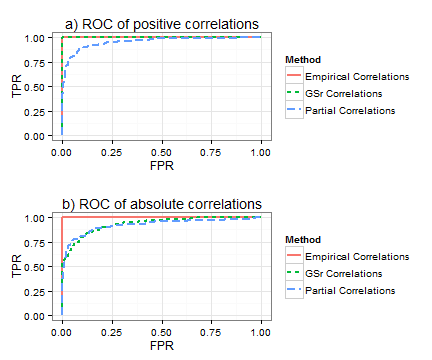
\includegraphics[width=\maxwidth]{GSFigs/GSROCnoGS} 

}

\caption[ROC plot assessing the ability of the empirical correlations, partial correlations and correlations after GS removal to separate the true zero correlations the a) true positive correlations b) true non-zero correlations]{ROC plot assessing the ability of the empirical correlations, partial correlations and correlations after GS removal to separate the true zero correlations the a) true positive correlations b) true non-zero correlations. Plotted here are the true positive rates (TPR), or the rate at which true non-zero correlations were detected as non-zero, against the false positive rates (FPR), or the rate at which true zero correlations were detected as non-zero, from a simulation without superimposed global signal.\label{fig:ROCnoGS}}
\end{figure}


\end{knitrout}






\clearpage
\subsection{Global Signal}

We now consider adding in a Global Signal to the simulation. This global signal is simply generated from a normal distribution with mean five and standard deviation one and then superimposed onto a simulated BOLD signal described earlier. In this simulation the global signal is assumed to affect all regions of the brain uniformly. The densities of the empirical correlations, partial correlations and correlations after GS removal are plotted in Figure \ref{fig:DensityGS}. Here as potentially expected we find that the empirical correlations still split the true connections and non-existant connections well however they are now not centered around there ``true" values as a large amount of positive correlation has been introduced into the system. The global signal removed correlations however are much closer to there true values, although still have been shifted negatively. The partial correlations appear unaffected by this superimposed global signal in comparison to the previous simulation.

In Figure \ref{fig:dotPlotGS} we again see that the global signal removed correlation exhibit a negative bias whilst the partial correlations on average are able to recapture their true values. In Figure \ref{fig:ROCGS} both the empirical correlations and global signal removed correlations are able to separate trully positive correlations from zero correlations. However, the global signal removed correlations now perform worse when separating true non-zero correlations from zero correlations.


\begin{knitrout}
\definecolor{shadecolor}{rgb}{0.969, 0.969, 0.969}\color{fgcolor}\begin{figure}[]


{\centering 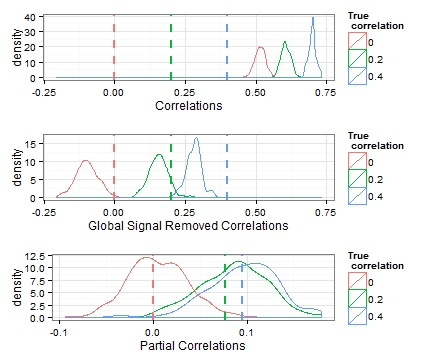
\includegraphics[width=\maxwidth]{GSFigs/GSDensityGS} 

}

\caption[The densities of the empirical correlations, partial correlations and correlations after GS removal are plotted for a simulation with a superimposed global signal]{The densities of the empirical correlations, partial correlations and correlations after GS removal are plotted for a simulation with a superimposed global signal. Correlations are labelled as to whether they were 0, 0.2 or 0.4 in the true correlation matrix that was used to generate them.\label{fig:DensityGS}}
\end{figure}


\end{knitrout}


\begin{knitrout}
\definecolor{shadecolor}{rgb}{0.969, 0.969, 0.969}\color{fgcolor}\begin{figure}[]


{\centering 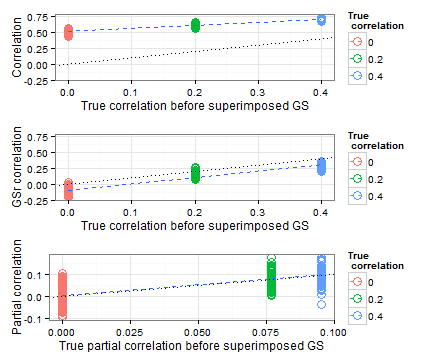
\includegraphics[width=\maxwidth]{GSFigs/GSdotPlotGS} 

}

\caption[The empirical correlations, partial correlations and correlations after GS removal from a simulation with a superimposed global signal are plotted against their true values]{The empirical correlations, partial correlations and correlations after GS removal from a simulation with a superimposed global signal are plotted against their true values. The black dotted line is the y=x line. The blue dashed line is the line of best fit from a linear regression.\label{fig:dotPlotGS}}
\end{figure}


\end{knitrout}


\begin{knitrout}
\definecolor{shadecolor}{rgb}{0.969, 0.969, 0.969}\color{fgcolor}\begin{figure}[]


{\centering 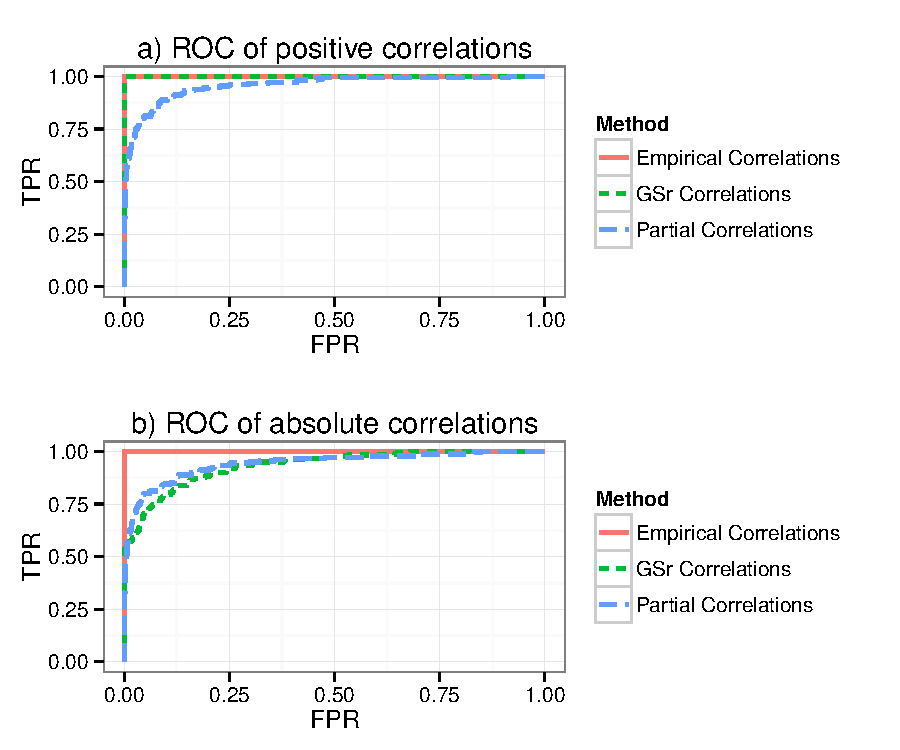
\includegraphics[width=\maxwidth]{GSFigs/GSROCGS} 

}

\caption[ROC plot assessing the ability of the empirical correlations, partial correlations and correlations after GS removal to separate the true zero correlations the a) true positive correlations b) true non-zero correlations]{ROC plot assessing the ability of the empirical correlations, partial correlations and correlations after GS removal to separate the true zero correlations the a) true positive correlations b) true non-zero correlations. Plotted here are the true positive rates (TPR), or the rate at which true non-zero correlations were detected as non-zero, against the false positive rates (FPR), or the rate at which true zero correlations were detected as non-zero, from a simulation with a superimposed global signal.\label{fig:ROCGS}}
\end{figure}


\end{knitrout}









\clearpage
\subsection{Areas Under the ROC Curves}

The information contained within the ROC curve plots from the previous simulations is summarised in Table \ref{auROC}. Table \ref{auROC} 
 summarised the areas under the ROC curve (AUC) for the two simulations and three methods. The larger the AUC value the better the method was at separating non-zero from zero correlations. Here we observe that correlation performs best when there is no global signal and when there is uniform global signal. The performance of Partial correlations improves when there is a global signal. Global signal removal causes trully zero correlations to be shifted negative, this creates a difficulty in separating non-zero from zero correlations if sign is not considered.
% latex table generated in R 3.1.0 by xtable 1.7-3 package
% Mon Nov 24 11:28:31 2014
\begin{table}[ht]
\centering
\begin{tabular}{rrrr}
  \hline
 & cor & partial.cor & GSr.cor \\ 
  \hline
no GS & 0.97 & 0.92 & 0.90 \\ 
  GS & 0.97 & 0.94 & 0.90 \\ 
   \hline
\end{tabular}
\caption{A table of the areas under the ROC curves for separating true non-zero from zero correlations. Two simulations are considered, one without a global signal and one with super-imposed global signal} 
\label{auROC}
\end{table}


\clearpage
\subsection{Relationship between average global signal and average correlation}

We next consider the relationship between average global signal and average correlation. To do this we perform 50 simulations of the uniform global signal simulation described earlier, where in each of these simulations a different amount of global signal is super-imposed onto the simulations. These results are plotted in Figure \ref{fig:avgGSavgCOR}. Here it is observed that as the amount of global signal in the system increases so does the average correlation.

\begin{knitrout}
\definecolor{shadecolor}{rgb}{0.969, 0.969, 0.969}\color{fgcolor}\begin{figure}[]


{\centering 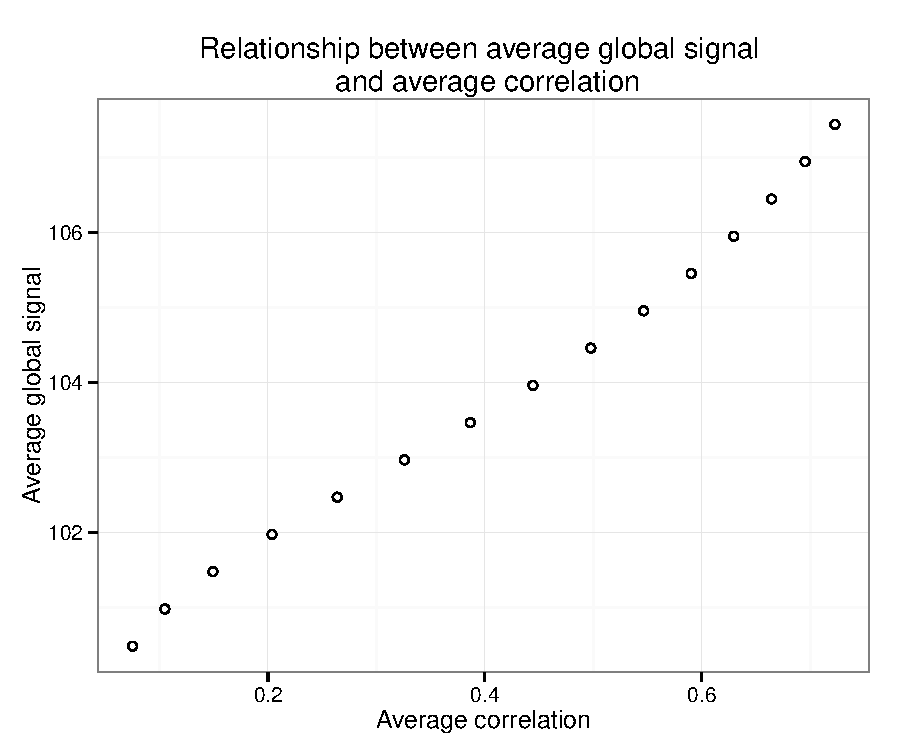
\includegraphics[width=\maxwidth]{GSFigs/GSavgGSavgCOR} 

}

\caption[A plot of the relationship between average global signal and average correlation for 50 simulations with varying amounts of super-imposed uniform global signal]{A plot of the relationship between average global signal and average correlation for 50 simulations with varying amounts of super-imposed uniform global signal\label{fig:avgGSavgCOR}}
\end{figure}


\end{knitrout}




\begin{knitrout}
\definecolor{shadecolor}{rgb}{0.969, 0.969, 0.969}\color{fgcolor}\begin{figure}[]


{\centering 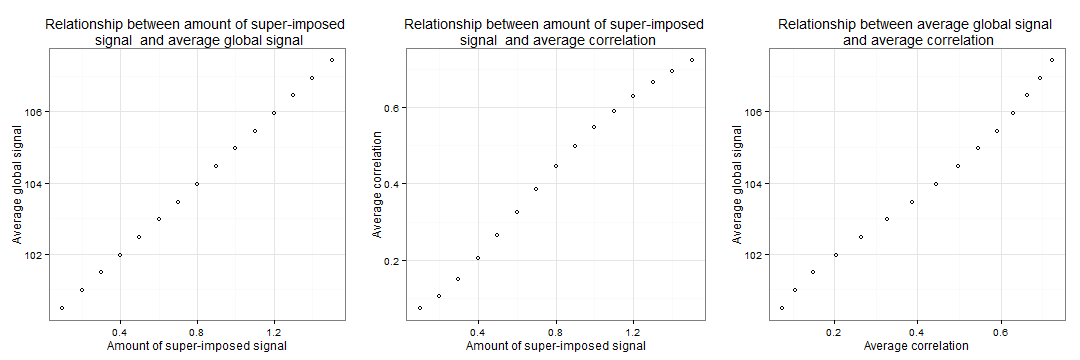
\includegraphics[width=\maxwidth]{GSFigs/GSGSCorandAmount} 

}

\caption[]{\label{fig:GSCorandAmount}}
\end{figure}


\end{knitrout}




\begin{knitrout}
\definecolor{shadecolor}{rgb}{0.969, 0.969, 0.969}\color{fgcolor}\begin{figure}[]


{\centering 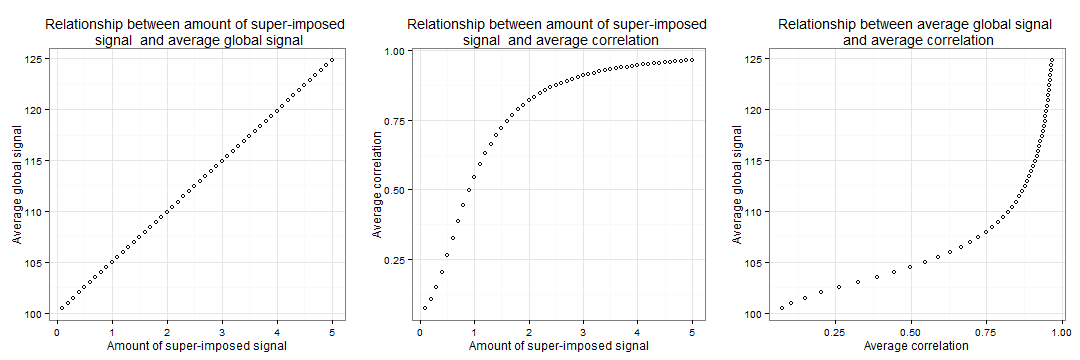
\includegraphics[width=\maxwidth]{GSFigs/GSGSCorandAmount2} 

}

\caption[]{\label{fig:GSCorandAmount2}}
\end{figure}


\end{knitrout}


\end{document}
